\begin{frame}
    \frametitle{Partie de Tiany}
    \centering
    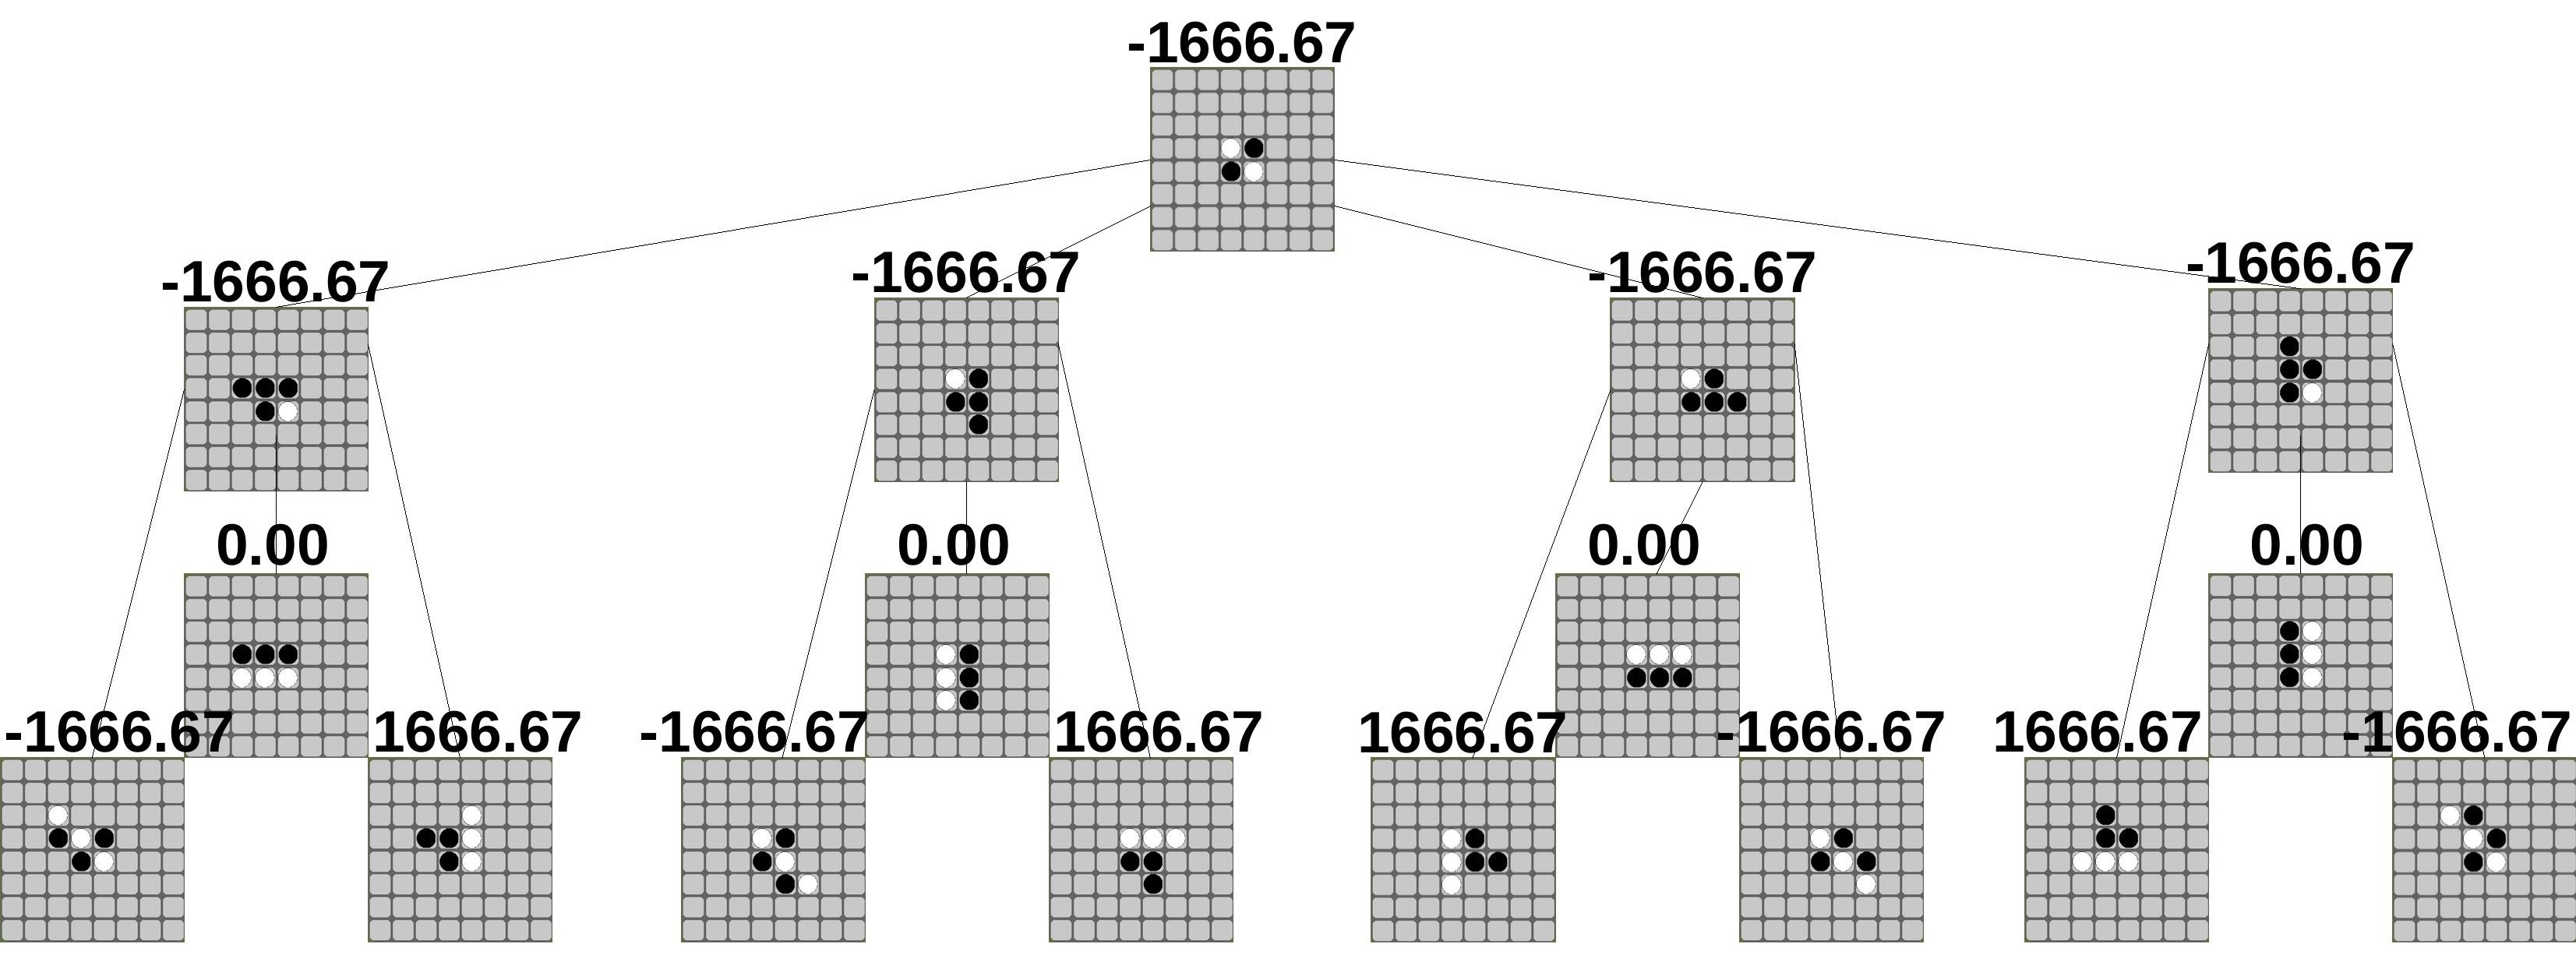
\includegraphics[width=0.8\textwidth]{img/minmax_eval.jpg}
\end{frame}

\begin{frame}[t]{Comment concevoir une méthode d'évaluation}
    \textbf{Stratégies pour gagner à Othello}
    \begin{itemize}
        \item Contrôle des coins 
        \item Contrôle des bords 
        \item Réduction de la mobilité de l'adversaire
    \end{itemize}
    \begin{center}
        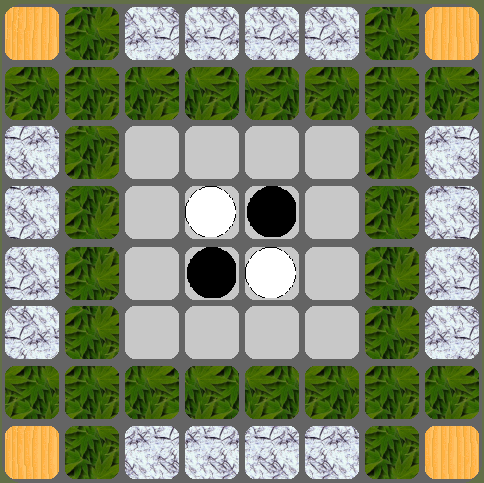
\includegraphics[width=0.3\textwidth]{img/eval_0.png}
    \end{center}
    \textbf{Les coins sont en or, les bords en argent, et le centre est dangereux}
\end{frame}

\begin{frame}[t,fragile]{Comment concevoir une méthode d'évaluation}
    \textbf{Première idée:}
    Une matrice de pondération
    \begin{lstlisting}[basicstyle=\scriptsize, escapeinside={(*}{*)}]
def evaluate_board(self, board) -> float:
    WEIGHTS = [
        [150, -50, 20, 10, 10, 20, -50, 150],
        [-50, -50, -2, -2, -2, -2, -50, -50],
        [20, -2, 1, 1, 1, 1, -2, 20],
        [10, -2, 1, 0, 0, 1, -2, 10],
        [10, -2, 1, 0, 0, 1, -2, 10],
        [20, -2, 1, 1, 1, 1, -2, 20],
        [-50, -50, -2, -2, -2, -2, -50, -50],
        [150, -50, 20, 10, 10, 20, -50, 150]
    ]
    
    score = 0
    for i in range(8):
        for j in range(8):
            if board.get_at(i, j) == board._current_player:
                score += WEIGHTS[i][j]
            elif board.get_at(i, j) == 1 - board._current_player:
                score -= WEIGHTS[i][j]
    return score
    \end{lstlisting}
\end{frame}
